\documentclass{article}
\PassOptionsToPackage{numbers,sort&compress}{natbib}
\usepackage[preprint]{neurips_2023}
\makeatletter
\renewcommand{\@noticestring}{}
\makeatother

\usepackage[utf8]{inputenc}
\usepackage[T1]{fontenc}
\usepackage{microtype}
\usepackage[hidelinks]{hyperref}
\usepackage{amssymb}
\usepackage{amsmath}
\usepackage{array,booktabs,longtable}
\usepackage{graphicx}
\usepackage{float}

\setcitestyle{numbers,square}
\title{JEP LLM Benchmarking Proposal}
\author{Peter Driscoll}
\begin{document}
\raggedbottom
\maketitle

\section{Introduction}
Transitional justice research uses qualitative coding to compare testimony~\cite{Schirmer2025}. In the Casanare case of Colombia's Special Jurisdiction for Peace (JEP)~\cite{JEPCaso03}, the focus of this study, accounts may be similar under one aspect and different under another. For example, testimony may express similar narratives of harm, yet diverge into very different narratives of reparation. Conditional semantic textual similarity (C-STS) formalizes this type of comparison by scoring the similarity of two passages on a 1--5 scale based on a condition relevant to both of them. This provides a quantitative target for learning representations that preserve these distinctions~\cite{C-STS}.

Reliance on consistent human annotations limits the scale at which researchers can analyze these corpora. LLMs have shown potential to reduce this reliance by automating text annotation, with demonstrated applications to political relevance and framing~\cite{Gilardi2023}.

However, studies do not consistently compare candidate models or validate model outputs against independent human annotations~\cite{Desai2026}. These gaps motivate our benchmarking study, which will compare open and closed-source LLMs with language and domain-adapted encoders to guide model selection for codebook development, passage retrieval, and passage classification of the Casanare subcase of JEP Case 03~\cite{JEPCaso03}. Experts from JEP will validate the resulting codebook, retrieved passages, and classifications.

\subsection{Preliminary evidence for conditional representations}
We compared control Qwen3-Embedding-8B with Qwen3-Embedding-8B fine-tuned on the conditional similarity objective. On the same 65 C-STS validation inputs, the fine-tuned model grouped sentences much more consistently by target color (Figure~\ref{fig:csts-color-clustering}). For example, the validation data pair ``shorts color'' with a man in red shorts entering water, and ``color of clothing'' with a boy in a blue shirt jumping into water. They fall into red and blue groups in the fine-tuned model, suggesting it is picking up the color asked for even when the scenes are similar. This supports testing the approach on JEP narratives~\cite{CSTSColorClustering}.

\begin{figure}[H]
\centering
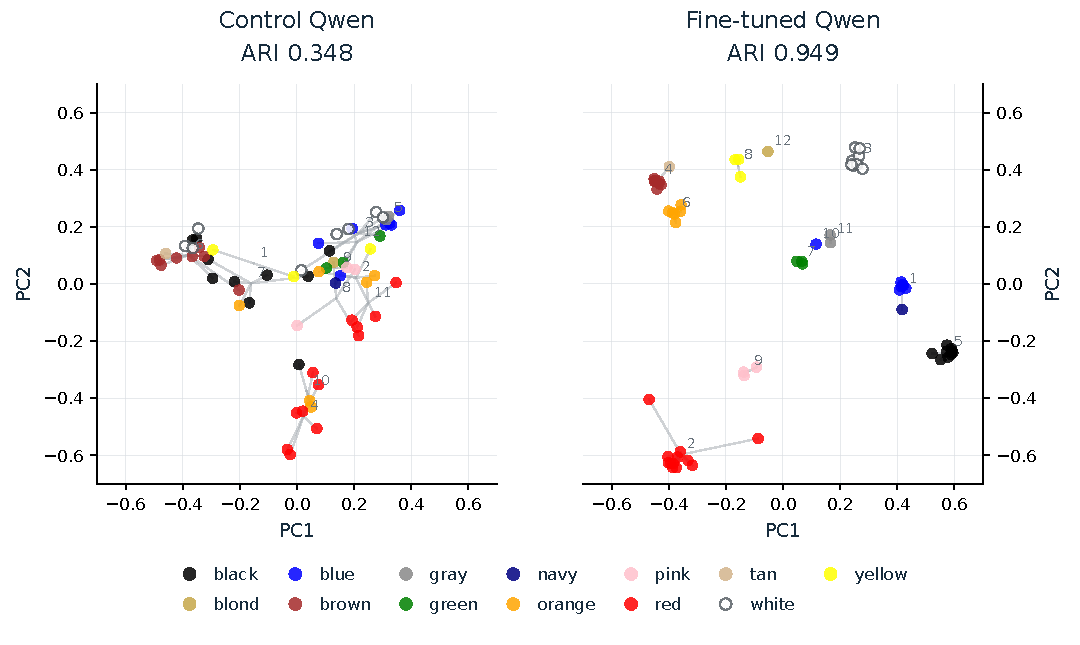
\includegraphics[width=\linewidth]{figures/qwen-k12-pca-comparison.pdf}
\caption{Fine-tuned Qwen (right) groups sentences by color more consistently than control Qwen (left), improving agreement with color labels (adjusted Rand index, ARI) from 0.348 to 0.949. Both panels show the same 65 C-STS sentences. Each dot uses the color of the item named in its condition, such as clothing; gray lines connect dots to cluster centers (\(K=12\)). Each panel uses its own PCA projection.}
\label{fig:csts-color-clustering}
\end{figure}

\section{Evaluation datasets}
\noindent\textbf{[WIP: Need to add the MET-D benchmark. Its task description, evaluation protocol, and scoring metrics remain to be specified.]}\par\smallskip

We will evaluate the models on nine benchmark datasets plus a JEP passage-retrieval evaluation: three general Spanish benchmarks, one Colombian Spanish benchmark, four Spanish crime and politics datasets used to evaluate ConfliBERT-Spanish~\cite{ConfliBERT-Spanish}, and one conditional semantic similarity dataset.

\subsection{General Spanish tasks}
\begin{itemize}
    \item \textbf{XL-Sum} tests summarization of Spanish news articles against human-written reference summaries~\cite{XL-SUM}.
    \item \textbf{MMLU-ProX-Lite} tests subject knowledge and reasoning through Spanish multiple-choice (MC) questions~\cite{MMLU-ProX-Lite}.
    \item \textbf{XQuAD} tests reading comprehension through questions answered using a supplied passage~\cite{XQuad}.
    \item \textbf{XCol} tests Colombian Spanish reading comprehension and legal reasoning using 183 questions from official educational and professional assessments~\cite{XCol}.
\end{itemize}

\subsection{Spanish crime and politics}

\begin{itemize}
    \item \textbf{Huffington Post} tests binary text classification of Spanish news articles as politically relevant or irrelevant, against labels derived from their editorial sections~\cite{ConfliBERT-Spanish}.
    \item \textbf{Protest} tests binary and multilabel text classification of Spanish news reports against reference annotations distinguishing verbal and material conflict and cooperation~\cite{ConfliBERT-Spanish}.
    \item \textbf{InsightCrime} tests multilabel text classification of Spanish crime reports against the four-label subset used by ConfliBERT-Spanish: law enforcement, drug trafficking, homicides, and corruption~\cite{ConfliBERT-Spanish}. The source corpus combines expert annotations with automated label propagation~\cite{Parolin2021}.
    \item \textbf{Mx-News} tests named entity recognition (NER) (Section~\ref{app:ner}) in Spanish political news against reference entity spans and 17 entity types labeled by one human annotator~\cite{MxNews}.
\end{itemize}

\subsection{English conditional semantic similarity}
C-STS tests similarity between sentence pairs under a specified condition, using our LLM-cleaned and validated revision 1.1~\cite{C-STSCleaned}.

\subsection{JEP passage retrieval}
Our team will read one randomly selected transcript from the held-out trial split for the Casanare subcase of JEP Case 03~\cite{JEPCaso03}. We will identify every passage concerning narratives of harm, reparation, restoration, or sanctions. Passages may belong to more than one narrative. LLMs and encoders will rank the same fixed passage pool (Section~\ref{app:retrieval}) for each narrative, with the aim of retrieving all relevant examples. Retrieval thresholds (Section~\ref{app:retrieval}) will be selected on separate validation material.

\section{Model candidates}
\subsection{Generative LLMs}
\subsubsection{Open source}
Fine-tuned Gemma-4 and fine-tuned Qwen3.8-27B~\cite{ModelDocs}.

\subsubsection{Closed source}
GPT-6.1 Sol at \texttt{max} reasoning effort, Claude Opus 5.5, and Gemini 4 Argon~\cite{ModelDocs}.

\subsection{Text encoder}
\subsubsection{Architectures}
We compare backbone families, attention masks, and independent versus joint passage encoding for condition steering in C-STS.
\begin{center}
\small
\begin{tabular}{@{}p{0.26\linewidth}p{0.36\linewidth}p{0.32\linewidth}@{}}
\toprule
\textbf{Model} & \textbf{Architecture} & \textbf{What it tests} \\
\midrule
Qwen3-Embedding-8B & Causal bi-encoder & Baseline embedding performance \\
Qwen3-Embedding-8B & Unmasked bidirectional bi-encoder & Effect of bidirectional attention \\
Qwen3-8B & Unmasked bidirectional cross-encoder & Joint condition--passage encoding \\
mDeBERTa-v3-base & Bidirectional bi-encoder & Dedicated encoder representation \\
mDeBERTa-v3-base & Bidirectional cross-encoder & Dedicated encoder joint scoring \\
\bottomrule
\end{tabular}
\end{center}

Qwen3-Embedding-8B establishes the causal embedding baseline~\cite{Qwen3-Embedding}. Its unmasked bi-encoder variant enables bidirectional attention over the condition and passage, following the decoder adaptation method of LLM2Vec~\cite{LLM2Vec}, holding pooling and scoring fixed. The unmasked Qwen3-8B cross-encoder jointly encodes the condition and both candidate passages, allowing each input token to attend to all other input tokens. \texttt{microsoft/mdeberta-v3-base}~\cite{DeBERTaV3} provides the dedicated encoder-only baseline, isolating independent passage encoding against joint scoring on a shared bidirectional backbone.

\subsection{Fine-tuning}
\subsubsection{Domain adaptation}
\noindent\textbf{[WIP: The MET-D adaptation, training targets, and evaluation criteria remain to be specified.]} We plan to fine-tune Qwen3.8-27B and Gemma-4 on other JEP subcases, adopting the MET-D framework for the JEP's definition of restorative justice.\par\smallskip

We will replicate ConfliBERT-Spanish-style continued pretraining using mDeBERTa-v3-base and the Spanish political-conflict corpus used by ConfliBERT-Spanish~\cite{ConfliBERT-Spanish}. We will compare the original and adapted checkpoints on the applicable benchmarks defined in this proposal. \emph{ConfliDeBERTaV3-Spanish} will denote our conflict-adapted mDeBERTa model.

Further adaptation of selected open models will use broad Colombian Spanish restorative-justice narratives and legal material, followed by narrower JEP testimony from other cases and adjacent Case 03 subcases. Comparisons before and after each stage will use the same subsequent task-training procedure~\cite{DomainAdaptivePretraining}. Casanare material will remain held out from training.

\subsubsection{Conditional contrastive}
\noindent\textbf{[WIP: This section still needs to be fleshed out.]} Spanish task training will compare seed-guided weak passage labels~\cite{XClass} with open-LLM-generated relevance labels. Conditional-comparison examples will pair passages under specified conditions. Specifically, contrastive learning evaluates passage pairs under a shared narrative condition: it clusters passages expressing similar accounts of that narrative and separates passages that diverge, penalizing superficial lexical overlap. Original passages with surrounding context and condition-focused summaries will be compared as alternative training inputs.

\section{Evaluation protocol}
Each candidate will be evaluated on the same fixed sample of 250 test items per applicable benchmark, or all items if fewer. JEP retrieval will use all passages in the randomly selected held-out transcript.

Scores are reported as follows:
\begin{itemize}
    \item XL-Sum: ROUGE-1, ROUGE-2, ROUGE-L F1 (Section~\ref{app:text-overlap})~\cite{XL-SUM,ROUGE}
    \item MMLU-ProX-Lite: MC accuracy (Section~\ref{app:accuracy})~\cite{MMLU-ProX-Lite}
    \item XQuAD: exact match (Section~\ref{app:accuracy}), token F1 (Section~\ref{app:text-overlap})~\cite{XQuad}
    \item XCol: MC accuracy (Section~\ref{app:accuracy})~\cite{XCol}
    \item Huffington Post: positive-class precision, recall, F1 (Section~\ref{app:prf})~\cite{ConfliBERT-Spanish}
    \item Protest: positive-class F1; macro and per-label F1 (Section~\ref{app:prf})~\cite{ConfliBERT-Spanish}
    \item InsightCrime: macro and per-label F1 (Section~\ref{app:prf})~\cite{ConfliBERT-Spanish,Parolin2021}
    \item Mx-News: entity micro F1 (Section~\ref{app:ner})~\cite{MxNews,CoNLL2003}
    \item C-STS: Spearman correlation, mean squared error, condition-ordering accuracy (Section~\ref{app:similarity})~\cite{C-STSCleaned}
    \item JEP retrieval: Recall@1/5/10, MRR@10, precision, recall, F1 (Section~\ref{app:retrieval})~\cite{IRMeasures}
\end{itemize}

LLM cost will be reported per token (Section~\ref{app:cost}).

\section{Appendix}
\subsection{Formulas}
\label{app:formulas}

\subsubsection{Accuracy}
\label{app:accuracy}
Accuracy is the fraction of answers that are correct. For \(n\) test items, let \(a_i=1\) if answer \(i\) is correct and \(a_i=0\) otherwise:
\[
\mathrm{Accuracy} = \frac{1}{n}\sum_{i=1}^{n} a_i.
\]
For MC questions, the selected option must match the answer key. For XQuAD, the complete answer must match an accepted reference after the benchmark's normalization; this is called exact-match answer accuracy~\cite{XQuad}.

\subsubsection{Precision, recall, and F1}
\label{app:prf}
Given \(n\) binary decisions, define the predicted labels and true labels:
\[
\hat{y},y \in \{0,1\}^n.
\]
Here, \(i\) indexes decisions and \(1\) denotes the positive class:
\[
\begin{aligned}
TP &= \left| \{ i \in \{1,\ldots,n\} : \hat{y}_i = 1 \land y_i = 1 \} \right|, \\
FP &= \left| \{ i \in \{1,\ldots,n\} : \hat{y}_i = 1 \land y_i = 0 \} \right|, \\
FN &= \left| \{ i \in \{1,\ldots,n\} : \hat{y}_i = 0 \land y_i = 1 \} \right|.
\end{aligned}
\]
Precision is the fraction of predicted positives that are correct:
\[
P = \frac{TP}{TP+FP}.
\]
Recall is the fraction of reference positives recovered:
\[
R = \frac{TP}{TP+FN}.
\]
F1 is the harmonic mean of precision and recall:
\[
F_1 = \frac{2PR}{P+R} = \frac{2TP}{2TP+FP+FN}.
\]
For these three measures, ratios with a zero denominator are assigned zero.

Binary classification reports the positive-class scores. Multilabel classification applies the same definitions separately to each label. For \(C\) labels, where \(c\) indexes labels, macro F1 averages the label scores; micro F1 pools their counts:
\[
F_1^{\mathrm{macro}} = \frac{1}{C}\sum_{c=1}^{C}F_{1,c},
\qquad
F_1^{\mathrm{micro}} =
\frac{2\sum_{c=1}^{C}TP_c}
{2\sum_{c=1}^{C}TP_c+\sum_{c=1}^{C}FP_c+\sum_{c=1}^{C}FN_c}.
\]
Protest (multilabel) and InsightCrime report macro F1 and scores for each label.

\subsubsection{Text overlap: XQuAD and ROUGE}
\label{app:text-overlap}
The same precision, recall, and F1 definitions apply to matching text units. Let \(m\) count matching units, \(a\) count predicted units, and \(b\) count reference units:
\[
P = \frac{m}{a}, \qquad R = \frac{m}{b}, \qquad
F_1 = \frac{2m}{a+b}.
\]
XQuAD uses normalized answer tokens, ignoring their order and counting repeated occurrences. Each answer receives its best score against the accepted references~\cite{XQuad}.

ROUGE compares generated summaries with reference summaries~\cite{ROUGE}. An \(n\)-gram is a sequence of \(n\) consecutive words. ROUGE-1 matches individual words; ROUGE-2 matches consecutive word pairs. ROUGE-L uses the length of the longest common subsequence: words appearing in the same order in both texts, with gaps allowed. We report the F1 form of each measure. XQuAD and XL-Sum scores are averaged over test items.
\subsubsection{XQuAD text normalization}
We will use the official SQuAD v1.1 scorer specified by XQuAD~\cite{XQuad}. It lowercases answers, removes ASCII punctuation and the English articles \emph{a}, \emph{an}, and \emph{the}, and normalizes whitespace. Token F1 then splits the normalized answers on whitespace. These rules also apply to the Spanish evaluation.

\subsubsection{NER and entity spans}
\label{app:ner}
NER identifies text spans and assigns entity types, such as person, organization, or location. A span is a contiguous stretch of text identified by its start and end positions. For example, in the sentence \emph{María López habló}, the two-word name \emph{María López} is a person span; predicting only \emph{López} gives different boundaries.

A predicted entity matches a reference only when its document, start and end positions, and type all agree~\cite{CoNLL2003}. Let \(\mathcal{E}_{\mathrm{pred}}\) and \(\mathcal{E}_{\mathrm{ref}}\) be the sets of predicted and reference entities across all documents and all 17 entity types:
\[
\begin{aligned}
TP &= |\mathcal{E}_{\mathrm{pred}} \cap \mathcal{E}_{\mathrm{ref}}|,\\
FP &= |\mathcal{E}_{\mathrm{pred}} \setminus \mathcal{E}_{\mathrm{ref}}|,\\
FN &= |\mathcal{E}_{\mathrm{ref}} \setminus \mathcal{E}_{\mathrm{pred}}|.
\end{aligned}
\]
Mx-News reports entity micro F1, which applies the precision, recall, and F1 formulas (Section~\ref{app:prf}) to these counts pooled across all 17 entity types and documents, rather than averaging per-type scores. A boundary or type error produces an unmatched prediction and an unmatched reference.

\subsubsection{Passage retrieval}
\label{app:retrieval}
For each narrative query \(q\), models rank the \textbf{fixed passage pool} \(\mathcal{P}\), containing all passages in the selected held-out Casanare transcript. Human annotators identify the reference set of relevant passages \(\mathcal{R}_q \subseteq \mathcal{P}\). Let \(\mathcal{D}_{q,k} \subseteq \mathcal{P}\) contain the first \(k\) retrieved passages. Recall@\(k\) measures the fraction of relevant passages recovered within those results~\cite{IRMeasures}:
\[
\mathrm{Recall}@k(q) =
\frac{|\mathcal{D}_{q,k}\cap\mathcal{R}_q|}{|\mathcal{R}_q|}.
\]
We report \(k\in\{1,5,10\}\). For \(Q\) narrative queries, let \(r_q\) be the rank of the first relevant passage, or infinity if none is retrieved. Mean reciprocal rank at 10 is~\cite{IRMeasures}:
\[
\mathrm{MRR}@10 =
\frac{1}{Q}\sum_{q=1}^{Q}
\begin{cases}
1/r_q, & r_q\leq 10,\\
0, & r_q>10.
\end{cases}
\]

For unranked retrieval, a score cutoff \(\tau\) acts as the \textbf{retrieval threshold}, selected on separate validation material to maximize F1. Passages with scores at or above \(\tau\) form the returned set. True positives are relevant passages retrieved, false positives are irrelevant passages retrieved, and false negatives are relevant passages missed; full-set precision, recall, and F1 use the same formulas (Section~\ref{app:prf}). Retrieval scores are reported per narrative and averaged equally across narratives. Recall is assigned zero when a narrative has no reference passages.

\subsubsection{Conditional similarity}
\label{app:similarity}
For \(n\) sentence pairs, let \(\hat{s}_i\) and \(s_i\) be the predicted and reference similarity scores for pair \(i\), each on the 1--5 scale. Mean squared error (MSE) is:
\[
\mathrm{MSE} = \frac{1}{n}\sum_{i=1}^{n}(\hat{s}_i-s_i)^2.
\]
For encoder MSE, we will fit an affine map \(az+b\) from raw similarity \(z\) to reference scores on the validation split by least squares, with slope \(a\geq 0\) and intercept \(b\in\mathbb{R}\)~\cite{LinearCalibration}. We will freeze both parameters before testing and clip predictions to the 1--5 range:
\[
\hat{s} = \min\{5,\max\{1,az+b\}\}.
\]
LLMs will return scores directly on the 1--5 scale. Spearman correlation will use raw encoder similarities and LLM scores.

Spearman correlation measures agreement between the rankings induced by predicted and reference scores~\cite{C-STS}. Let \(u_i\) and \(v_i\) be the ranks of raw model scores and reference scores, respectively, with tied scores assigned average ranks, and let \(\bar{u}\) and \(\bar{v}\) be the mean ranks:
\[
\rho =
\frac{\sum_{i=1}^{n}(u_i-\bar{u})(v_i-\bar{v})}
{\sqrt{\left[\sum_{i=1}^{n}(u_i-\bar{u})^2\right]
\left[\sum_{i=1}^{n}(v_i-\bar{v})^2\right]}}.
\]
Spearman correlation is undefined if either ranking has no variation.

Condition-ordering accuracy measures whether the model correctly ranks pairs of conditions with distinct reference ratings for the same passage pair. For all \(M\) condition pairs on an identical passage pair with reference ratings \(y_a \neq y_b\), let \(\hat{s}_a\) and \(\hat{s}_b\) be the predicted scores. Pairs where \((\hat{s}_a - \hat{s}_b)(y_a - y_b) > 0\) receive full credit, while tied predictions receive half credit:
\[
\mathrm{Acc}_{\mathrm{cond}} = \frac{1}{M}\sum_{j=1}^{M} \left[ \mathbb{I}\left((\hat{s}_a - \hat{s}_b)(y_a - y_b) > 0\right) + 0.5 \cdot \mathbb{I}\left(\hat{s}_a = \hat{s}_b\right) \right].
\]

\subsubsection{Token cost}
\label{app:cost}
Token cost is the billed amount per token. Input and output token costs are reported separately using each provider's pricing~\cite{ModelDocs}.

\subsection{Task examples}
\label{app:examples}
These examples and target outputs are constructed illustrations. Bold text marks answer or entity spans.

\begingroup
\small
\hbadness=10000
\setlength{\LTleft}{0pt}
\setlength{\LTright}{0pt}
\setlength{\parskip}{8pt}
\renewcommand{\arraystretch}{1.5}
\begin{longtable}{@{}>{\raggedright\arraybackslash\setlength{\parskip}{4pt}}p{\dimexpr0.54\linewidth-\tabcolsep\relax}>{\raggedright\arraybackslash\setlength{\parskip}{4pt}}p{\dimexpr0.46\linewidth-\tabcolsep\relax}@{}}
\toprule
\textbf{Input} & \textbf{Question and target output} \\
\midrule
\endfirsthead
\toprule
\textbf{Input} & \textbf{Question and target output} \\
\midrule
\endhead
\bottomrule
\endfoot
\bottomrule
\endlastfoot

\textbf{XL-Sum}~\cite{XL-SUM}\par
El municipio abrirá dos bibliotecas en junio. Tendrán acceso gratuito y ofrecerán talleres de lectura los fines de semana. El proyecto busca ampliar los espacios educativos de los barrios.
&
\textit{Target summary}\par
El municipio abrirá en junio dos bibliotecas gratuitas con talleres de lectura.
\\
\midrule

\textbf{MMLU-ProX-Lite}~\cite{MMLU-ProX-Lite}\par
Una bolsa contiene tres bolas rojas y dos azules. Si se extrae una bola al azar, ¿cuál es la probabilidad de que sea roja?\par
A) \(1/5\); B) \(2/5\); C) \(3/5\); D) \(4/5\); E) \(1/2\); F) \(1/3\); G) \(2/3\); H) \(1/4\); I) \(3/4\); J) \(1\).
&
\textit{Correct option}\par
C) \(3/5\).
\\
\midrule

\textbf{XQuAD}~\cite{XQuad}\par
La biblioteca municipal abrió en \textbf{2018}. Tiene una sala infantil y un archivo de historia local. Los talleres de lectura se realizan los sábados.
&
\textit{Question}\par
¿En qué año abrió la biblioteca municipal?\par
\textit{Answer span}\par
2018.
\\
\midrule

\textbf{XCol}~\cite{XCol}\par
Una alcaldía abre una consulta ciudadana sobre el uso de un parque. Solo publica la convocatoria en una plataforma que requiere conexión a internet.
&
\textit{Question}\par
¿Qué cambio facilitaría la participación de personas sin acceso a internet?\par
A) Acortar el plazo.\newline
B) Recibir propuestas también de forma presencial.\newline
C) Exigir una contraseña más larga.\newline
D) Limitar el número de propuestas.\par
\textit{Correct option:} B.
\\
\midrule

\textbf{Huffington Post}~\cite{ConfliBERT-Spanish}\par
El Congreso debatió la reforma electoral durante una sesión extraordinaria. Representantes de varios partidos presentaron sus propuestas.
&
\textit{Reference label}\par
Politically relevant.\par
The label is derived from the article's editorial section, \emph{Política}.
\\
\midrule

\textbf{Protest}~\cite{ConfliBERT-Spanish}\par
Los manifestantes bloquearon la carretera y denunciaron públicamente la actuación del gobierno.
&
\textit{Binary label}\par
Conflict.\par
\textit{Multilabel output}\par
Material conflict; verbal conflict.
\\
\midrule

\textbf{InsightCrime}~\cite{Parolin2021}\par
La policía detuvo a tres integrantes de una red que transportaba cocaína e incautó el cargamento.
&
\textit{Labels}\par
Law enforcement; drug trafficking.
\\
\midrule

\textbf{Mx-News}~\cite{MxNews}\par
\textbf{María López} habló ante el \textbf{Congreso} en \textbf{Bogotá}.
&
\textit{Entity spans and types}\par
María López: PER (person).\newline
Congreso: ORG (organization).\newline
Bogotá: GPE (city).
\\
\midrule

\textbf{C-STS}~\cite{C-STS,C-STSCleaned}\par
\textit{Sentence 1}\par
A woman in a green coat is riding a bicycle.\par
\textit{Sentence 2}\par
A woman in a red coat is riding a bicycle.
&
\textit{Condition and illustrative score}\par
The activity described: \(5/5\).\par
The colour of the coat: \(1/5\).\par
The same pair receives different scores depending on the condition.
\\
\midrule

\textbf{JEP passage retrieval}~\cite{JEPCaso03}\par
P1: Desde entonces tengo pesadillas todas las noches.\par
P2: Pedimos una indemnización económica.\par
P3: Proponemos recuperar el lugar de encuentro de la comunidad.\par
P4: Pedimos una sanción para los responsables.\par
P5: Todavía no puedo trabajar por el dolor.
&
\textit{Narrative query \(\rightarrow\) relevant passages}\par
Harm \(\rightarrow\) P1, P5.\par
Reparation \(\rightarrow\) P2.\par
Restoration \(\rightarrow\) P3.\par
Sanctions \(\rightarrow\) P4.\par

\\
\end{longtable}
\endgroup

\clearpage
\begin{thebibliography}{99}
\small
\setlength{\itemsep}{1pt}
\bibitem{Schirmer2025} M.~Schirmer, J.~Pfeffer, and S.~Hilbert. \href{https://doi.org/10.1177/15586898231218463}{\emph{Talking About Torture: A Novel Approach to the Mixed Methods Analysis of Genocide-Related Witness Statements in the Khmer Rouge Tribunal}}. Journal of Mixed Methods Research, 19(1):83--102, 2025.
\bibitem{JEPCaso03} Jurisdicci\'on Especial para la Paz. \href{https://www.jep.gov.co/macrocasos/caso03.html}{\emph{Caso 03: Asesinatos y desapariciones forzadas presentados como bajas en combate por agentes del Estado}}. Official case overview and Casanare hearing recordings. Consulted November 3, 2026.
\bibitem{C-STS} A.~Deshpande et al. \href{https://aclanthology.org/2023.emnlp-main.345/}{\emph{C-STS: Conditional Semantic Textual Similarity}}. Proceedings of EMNLP, pp.~5669--5690, 2023.
\bibitem{Gilardi2023} F.~Gilardi, M.~Alizadeh, and M.~Kubli. \href{https://doi.org/10.1073/pnas.2305016120}{\emph{ChatGPT Outperforms Crowd Workers for Text-Annotation Tasks}}. Proceedings of the National Academy of Sciences, 120(30):e2305016120, 2023.
\bibitem{Desai2026} M.~Desai, D.~Card, and A.~Z.~Jacobs. \href{https://arxiv.org/abs/2607.07915}{\emph{Validating LLMs in Social Science: Epistemic Threats and Emerging Norms}}. arXiv:2607.07915, 2026.
\bibitem{CSTSColorClustering} P.~Driscoll. \href{https://github.com/pvd232/JEP/blob/9efa1d385fcc67f4daabc7f606f83263e8cdba0a/training_outputs/color_clustering_20261104/report.md}{\emph{C-STS Color Clustering Results}}. 2026. \href{https://github.com/pvd232/JEP/blob/9efa1d385fcc67f4daabc7f606f83263e8cdba0a/training_outputs/color_clustering_20261104/key_charts/matched-k/README.md}{Matched-\(K\) comparison and figure notes}; \href{https://github.com/pvd232/JEP/blob/9efa1d385fcc67f4daabc7f606f83263e8cdba0a/training_outputs/proposition_full_20261026/comparison_report.md}{encoder training protocol}.
\bibitem{ConfliBERT-Spanish} W.~Yang et al. \href{https://doi.org/10.1109/CiSt56084.2023.10409883}{\emph{ConfliBERT-Spanish: A Pre-trained Spanish Language Model for Political Conflict and Violence}}. 2023 7th IEEE Congress on Information Science and Technology (CiSt), pp.~287--292, 2023, especially Section III.
\bibitem{XL-SUM} T.~Hasan et al. \emph{XL-Sum: Large-Scale Multilingual Abstractive Summarization for 44 Languages}. 2021. \href{https://huggingface.co/datasets/csebuetnlp/xlsum}{Dataset card}, Spanish configuration.
\bibitem{MMLU-ProX-Lite} W.~Xuan et al. \href{https://arxiv.org/abs/2503.10497}{\emph{MMLU-ProX: A Multilingual Benchmark for Advanced Large Language Model Evaluation}}. 2025. \href{https://huggingface.co/datasets/li-lab/MMLU-ProX-Lite}{MMLU-ProX-Lite dataset card}, Spanish configuration.
\bibitem{XQuad} M.~Artetxe, S.~Ruder, and D.~Yogatama. \href{https://arxiv.org/abs/1910.11856}{\emph{On the Cross-lingual Transferability of Monolingual Representations}}. 2019 preprint. \href{https://github.com/google-deepmind/xquad}{XQuAD data and evaluation documentation}.
\bibitem{XCol} P.~Driscoll. \href{https://huggingface.co/datasets/pvd232/XCo}{\emph{Colombian Spanish Assessment Benchmark (XCol)}}. Version 1.0, 183-question TEST set, 2026.
\bibitem{Parolin2021} E.~S.~Parolin, L.~Khan, J.~Osorio, P.~T.~Brandt, V.~D'Orazio, and J.~Holmes. \href{https://doi.org/10.1109/DSAA53316.2021.9564232}{\emph{3M-Transformers for Event Coding on Organized Crime Domain}}. IEEE DSAA, pp.~1--10, 2021, Section IV.
\bibitem{MxNews} O.~Ramos-Flores et al. \href{https://doi.org/10.3233/JIFS-179868}{\emph{Probabilistic vs Deep Learning Based Approaches for Narrow Domain NER in Spanish}}. Journal of Intelligent \& Fuzzy Systems, 39(2):2015--2025, 2020. \href{https://github.com/orlandxrf/spanish-ner}{Author's dataset documentation}, Mx-news annotation details.
\bibitem{C-STSCleaned} P.~Driscoll. \href{https://github.com/pvd232/JEP/tree/main/datasets/csts-jep-revision-v1-1}{\emph{JEP C-STS Revision 1.1}}, 2026.
\bibitem{ModelDocs} Official model documentation: \href{https://developers.openai.com/api/docs/models/gpt-6.1-sol}{OpenAI GPT-6.1 Sol}; \href{https://platform.claude.com/docs/en/models/opus-5-5/overview}{Anthropic Claude Opus 5.5}; \href{https://ai.google.dev/gemini-api/docs/models/gemini-4-argon}{Google Gemini 4 Argon}; \href{https://ai.google.dev/gemma/docs/core/model_card_4}{Gemma 4}; \href{https://huggingface.co/Qwen/Qwen3.8-27B}{Qwen3.8}. Consulted November 3, 2026.
\bibitem{Qwen3-Embedding} Y.~Zhang et al. \href{https://arxiv.org/abs/2506.05176}{\emph{Qwen3 Embedding: Advancing Text Embedding and Reranking Through Foundation Models}}. 2025. \href{https://huggingface.co/Qwen/Qwen3-Embedding-8B}{Qwen3-Embedding-8B model card}.
\bibitem{DeBERTaV3} P.~He, J.~Gao, and W.~Chen. \href{https://arxiv.org/abs/2111.09543}{\emph{DeBERTaV3: Improving DeBERTa Using ELECTRA-Style Pre-Training with Gradient-Disentangled Embedding Sharing}}. ICLR, 2023.
\bibitem{ROUGE} C.-Y.~Lin. \href{https://aclanthology.org/W04-1013/}{\emph{ROUGE: A Package for Automatic Evaluation of Summaries}}. Text Summarization Branches Out, pp.~74--81, 2004.
\bibitem{CoNLL2003} E.~F.~Tjong Kim Sang and F.~De Meulder. \href{https://aclanthology.org/W03-0419/}{\emph{Introduction to the CoNLL-2003 Shared Task: Language-Independent Named Entity Recognition}}. Proceedings of CoNLL, pp.~142--147, 2003.
\bibitem{IRMeasures} ir\_measures contributors. \href{https://ir-measur.es/en/latest/measures.html}{\emph{Measure definitions: Recall@k, reciprocal rank, and set precision, recall, and F1}}. Project documentation. Consulted November 4, 2026.
\bibitem{LinearCalibration} scikit-learn developers. \href{https://scikit-learn.org/stable/modules/generated/sklearn.linear_model.LinearRegression.html}{\emph{LinearRegression}}. Official documentation: least-squares regression with an intercept and non-negative coefficients. Consulted November 4, 2026.
\bibitem{LLM2Vec} P.~BehnamGhader et al. \href{https://arxiv.org/abs/2404.05961}{\emph{LLM2Vec: Large Language Models Are Secretly Powerful Text Encoders}}. arXiv:2404.05961, 2024.
\bibitem{DomainAdaptivePretraining} S.~Gururangan et al. \href{https://aclanthology.org/2020.acl-main.740/}{\emph{Don't Stop Pretraining: Adapt Language Models to Domains and Tasks}}. Proceedings of ACL, pp.~8342--8360, 2020.
\bibitem{XClass} Z.~Wang, D.~Mekala, and J.~Shang. \href{https://aclanthology.org/2021.naacl-main.242/}{\emph{X-Class: Text Classification with Extremely Weak Supervision}}. Proceedings of NAACL-HLT, pp.~3043--3053, 2021.
\end{thebibliography}
\end{document}
